\section{In-match Server Features}
\label{sec:sprint3-gameserver}

In addition to matchmaking, some features needed by the server during a match was also planned. In particular, we would like to be able to check whether or not a person is staying on his route. There are several interesting problems in performing such a check, including routes that are not straight lines, and geometry using latitude and longitude. The solution for these problems are described in this section.

\subsection{Decimal Degree Geometry}
When working with coordinates in the Google Maps \ac{API}, a position is denoted as a set of \texttt{(Longitude, Latitude)}, also known as decimal degrees, upon the surface of the earth. This poses two problems when calculating distances between two arbitrary points.

The first problem is that the earth is a sphere, which means that conventional Euclidean geometry will not be correct. However, since the server will have to do a lot of computations, we decided that 100\% precision was not required for this (for example, whether you are 22 meters or 23 meters off route does not really matter), we decided to convert points to an offset in meters from \texttt{(Longitude, Latitude)} = \texttt{(0, 0)}, and then use Euclidean geometry on the resulting points.

That leads to the second problem. One degree of longitude's length in meters varies depending on the latitude~\citep{wikidecimaldegrees}. This meant a function, seen in \autoref{lst:sprint3-coord-offset}, had to be created to convert from coordinates in \texttt{(Longitude, Latitude)} to an \texttt{(x, y)} offset in meters. This approach resulted in very small imprecisions (on a scale of centimeters), though imprecisions grow as you get further from the equator.

\begin{code}[label={lst:sprint3-coord-offset}, caption={Convert Decimal Degrees to Offset in Meters}, language={Python}]
def metric_offset(coord):
	return (coord[0] * 111319.9 * cos(radians(coord[1])), coord[1] * 111319.9)
\end{code}

\subsection{Distance Between Point and Route}
Finding the distance between two points is not enough to determine whether a point is close to a route. The first problem with this, is that there might be quite far between two waypoints on a route, that is a user might have a 5 kilometre long route with just two waypoints. The natural solution to this is to project the point onto the line between the points and find the distance between those. However, as seen in \autoref{fig:sprint3-bad-route} using the line between the waypoints is often not indicative of the actual route.

\begin{figure}[!ht]
	\centering
	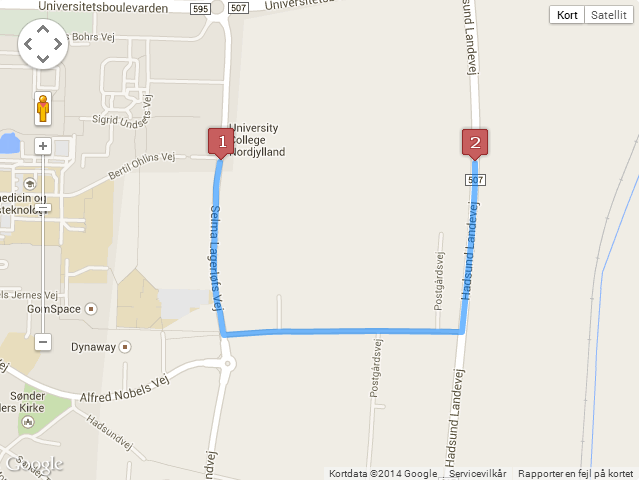
\includegraphics[scale=0.5]{img/sprint3br.png}
	\caption{Non-Linear Route}
	\label{fig:sprint3-bad-route}
\end{figure}

\subsubsection{Decoding the Route}
The solution we chose for that problem, was to use drawn line from the Google Maps Directions Service as the route, instead of the waypoints. This line is known as a polyline, and is returned with every successful request to the directions service. As mentioned in \autoref{sec:sprint2-web}, the web server already sends a directions request for each route, so even though it is not being drawn anywhere, the server has access to this polyline. 

Additionally, the polyline retrieved from the map API is encoded as a string, which can easily be stored in the database, giving the match server access to the line without sending requests to the Google Maps \ac{API}. It is possible to decode this line into a series of points. We decided to do this using an existing piece of open source Python2 code~\citep{decodepolyline}, which was ported to Python3. This function takes an encoded polyline and returns a list of \texttt{(Longitude, Latitude)} coordinates, which conveniently can be converted to the offsets we decided to work with, using the function seen in \autoref{lst:sprint3-coord-offset}. We denote these offsets for a given route ``checkpoints'', and store them in a class called \texttt{Polyline}.

\subsubsection{Distance to a Point}
A route's checkpoints represent the interval between each section of the route that can be represented as a straight line. That is, while the route in \autoref{fig:sprint3-bad-route} only has two waypoints, it has at least 4 checkpoints: The start, the end, and the two sharp turns. That means that as long as a users position is within some threshold of the lines between the checkpoints, he is on the correct route. To find out whether this is the case for a given position, several steps were implemented:

\begin{enumerate}
	\item{Convert the position to an offset in meters, called \texttt{point}.}
	\item{For each pair of consecutive waypoints on the route, define a \texttt{segment} starting at one of them and ending at the other.}
	\item{For each \texttt{segment}, find the shortest \texttt{distance} to \texttt{point}. The method chosen for this is described in more detail below.}
	\item{The shortest \texttt{distance} found is the distance from the point to the route.}
\end{enumerate}

When finding the distance between a line segment and a point, the method is as follows: Find out if the point is between the ends of the segments. If it is, project the point onto the line and take that distance. If it isn't, take the distance to the closest of the start and end points. This is illustrated in \autoref{fig:sprint3-linesegment}. This is not a new problem, and there were a lot of inspiration for efficient implementations of this to be found~\citep{point2line1,point2line2}, and we ended up with the functions seen in \autoref{lst:sprint3-dist}, a direct python implementation of referenced algorithms.

\begin{figure}[!ht]
	\centering
	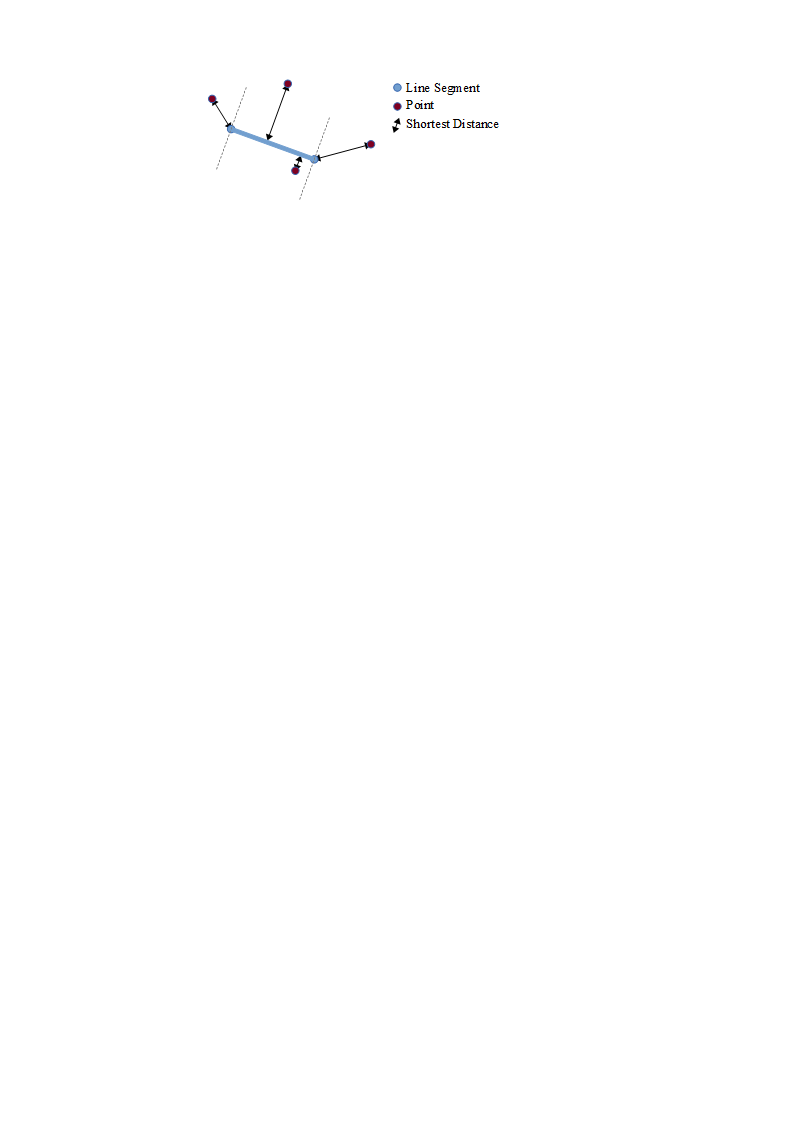
\includegraphics[scale=0.85]{img/sprint3linesegment.png}
	\caption{Shortest Distance to Line Segment}
	\label{fig:sprint3-linesegment}
\end{figure}

\begin{code}[label={lst:sprint3-dist}, caption={Distance Between Point and Line Segment}, language={Python}, style={PythonDoc}]
def dist2(p1, p2):
	return sqr(p1[0] - p2[0]) + sqr(p1[1] - p2[1])

def distToSegmentSquared(point, start, end):
	l2 = dist2(start, end)
	if l2 == 0:
		return 0

	'''
	t is position between start and end.
	Between 0 and 1 means the point is between start and end,
	less than 0 means before start and more than 1 means after end.
	'''
	t = ((point[0] - start[0]) * (end[0] - start[0]) + (point[1] - start[1]) * (end[1] - start[1])) / l2
	if t < 0:
		return dist2(point, start)
	elif t > 1:
		return dist2(point, end)
	else:
		return dist2(point, (start[0] + t * (end[0] - start[0]),
		                     start[1] + t * (end[1] - start[1])))

class Segment(object):
	def __init__(self, start, end):
		self.start = start
		self.end = end

	def point_distance(self, point):
		return sqrt(distToSegmentSquared(point, self.start, self.end))
\end{code}

With this, it was possible to implement a function for the \texttt{Polyline} class that given a route, a point and a threshold in meters is able to return whether or not the point is within threshold distance of the route. This can be used by the server to ensure that each participant in a match stays on their chosen route. The final implementation of the \texttt{Polyline} class can be seen in \autoref{lst:sprint3-polyline}. This in itself is not enough to check whether a participant is reaching checkpoints in the correct order, but is still an important part of the anti-cheating systems needed for the project.

\begin{code}[label={lst:sprint3-polyline}, caption={The \texttt{Polyline} Class}, language={Python}, style={PythonDoc}]
class Polyline(object):
	def __init__(self, encoded):
		# 'depoly' is the function to decode polyline strings.
		coords = depoly(encoded)
		self.points = [self.metric_offset(c) for c in coords]

	def metric_offset(self, coord):
		return (coord[0] * 111319.9 * cos(radians(coord[1])), coord[1] * 111319.9)

	def point_distance(self, coord):
		point = self.metric_offset(coord)
		distance = float('inf')
		for segment in self.get_segments():
			d = segment.point_distance(point)
			if (d < distance):
			distance = d
		return distance

	def get_segments(self):
		segments = []
		for i in range(len(self.points) - 1):
			segments.append(Segment(self.points[i], self.points[i+1]))
		return segments

	'''
	Checks whether a coordinate in (longitude, latitude) is within threshold in meters of the polyline.
	'''
	def on_route(self, coord, threshold = 50):
		return self.point_distance(coord) <= threshold
\end{code}
